\chapter{Literature Review}
\section{Topic Model}  
A topic model is a statistical tool that produce a short description of an original document. Topic models can be applied on a single document or a collection of documents. Blei (2012) described topic models as algorithms that discovers the main themes existing in a large text or document and otherwise the combination of two or more documents. He further reveal that the development of probabilistic topic modelling by ML  researchers as a set of algorithms that is geared towards revealing and describing large archives of documents with thematic information. Topic models analyses words in the large text document to discover the themes that pervades them, the connection that exist between the words and their with time. In topic modelling the stress of having to label the documents prior to annotations is saved as it is been done in supervised learning. from the analysis of the original document the topics are obtained. Given an very large volume of electronic archives that is impossible for human annotations, topic modelling can help to summarize and organize it.
\section{Topic Model methods}
Topic modelling techniques have been developed to automatically summarize document or large text. These techniques are: latent semantic indexing/allocation  (LSI/LSA), the latent dirichlet allocation (LDA) and the probabilistic latent semantic analysis (PLSA) . This research will narrow between LDA and LSA.
\section{Latent Semantic Analysis} 
Also known as the latent semantic indexing (LSI) is a topic model method
that transforms documents of high dimension to low dimension of words. One useful role played by LSI in topic modelling is its ability to deal with polysemy (Griffiths, Steyvors, 2006). Polysemy is a term that describes words with multiple meaning.
\section{How The LSA Works}
Preliminarily it constructs a matrix $M\in \mathbb{R}^{k*n}$, from the documents $d_1, d_2,..., d_k$ of words $w_1, w_2, ... w_n$. The rows represents the different words and the columns can be viewed as different documents. For example from \eqref{table:Table 2.1}, $m_{ij}$ shows the position and the frequency of the word $w_j$ in document $d_i$.
.To achieve reduction in the dimension of the matrix $M$ the truncated Singular Value Decomposition is applied, given as $M\approx A_t \sum B^{T}_t.$
$A_t$ and $B^T$ are orthogonal matrices, whilst $ \sum$ is a diagonal matrix.
Reducing the dimension leads to reduction of noise (Deerwester et al, 1990).
To achieve document similarity computing the dot product of the row vectors yields desired results.
\captionof{table}{Corpus of documents}
$$\begin{array}{cccc}
 &d_1 & d_2 &d_3 \\ 
 \text{food} & 0 & 0 & 2 \\ 
 \text{food} & 2 & 5 & 0 \\ 
 \text{cash} & 0 & 1 & 0 \\ 
 \text{automobile} & 1 & 0 & 4
\end{array} $$
%$$\text{fig. 1}$$
\section{ The Idea Latent Dirithchet Allocation}
 Blei(2012) referred to LDA as the simplest topic model . The ideas underlying this model is every document has several topics existing in it.He defined topic to be a distribution over a fixed a topic.Each topic is made up of words that are very related to the topic. Considering an article with a title "Seeking Life’s Bare (Genetic) Necessities,” for which data analysis was used to determine the number of genes an organism needs to survive. By hand words pertaining to three different vocabularies were highlighted with different colours. Words such as computer, prediction linked to the topic data analysis highlighted blue, life and evolve about evolutionary biology highlighted pink and words like gene, DNA describing the topic genetics is highlighted yellow. Stop words that occur frequently in the article are removed. 
The LDA as a statistical tool uses this idea with the assumption that topics are generated prior to words assignment. All words in each vocabulary has a probability value and depending on the topic each word finds itself would be high or low. For example the word "gene" will have a low probability value if it is in the domain of the  vocabulary "data analysis" compared to when it belongs to the topic "genetics".He described the process of assigning words in the document to each 
vocabulary as:
\begin{itemize}
\item[1.] From the documents a random distribution over topics is chosen.
\item[2.] for each word in the documents:
		\item[2a.]Randomly choose a topic from
the distribution over topics in step 1.
		\item[2b.]Randomly choose a word from the
corresponding distribution over
the vocabulary.
\end{itemize}
The LDA model reflects the idea of multiple topics exhibited by documents.
Figure  gives a picture of the whole intuition of this generative probabilistic process:

\begin{figure}[hbtp]
\centering
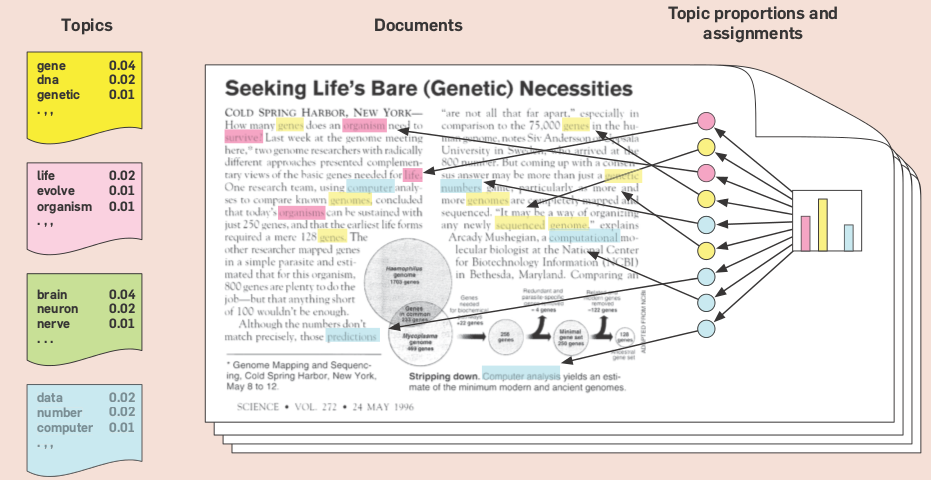
\includegraphics[scale=0.5]{DLA.png}
\caption{Generative intuition of LDA model}\label{Figure 2.1}
\end{figure}
In short description of Figure \eqref{Figure 2.1} the idea underlying LDA is that, first of all some number of topics that are distribution over words is assumed (far left). In generating for each document, firstly choose a distribution over topics (far right ie. histogram), then the circles of different colours are topic assignment for which words drawn from the document corresponds to.

Figure \eqref{Figure 2.2} shows real inference with LDA, using 17000 articles from the journal of science. Genetics, Evolution, Disease and Computers represents the topics from one article and the words below each are top 15 most frequent words. The graph on the left shows the probability values for each topic.
The probability values for this article for a given set of topics may be different from another article. in effect, even though some documents or articles may share the same topics, each article exhibits the topics in different proportions.
\begin{figure}[hbtp]
\centering
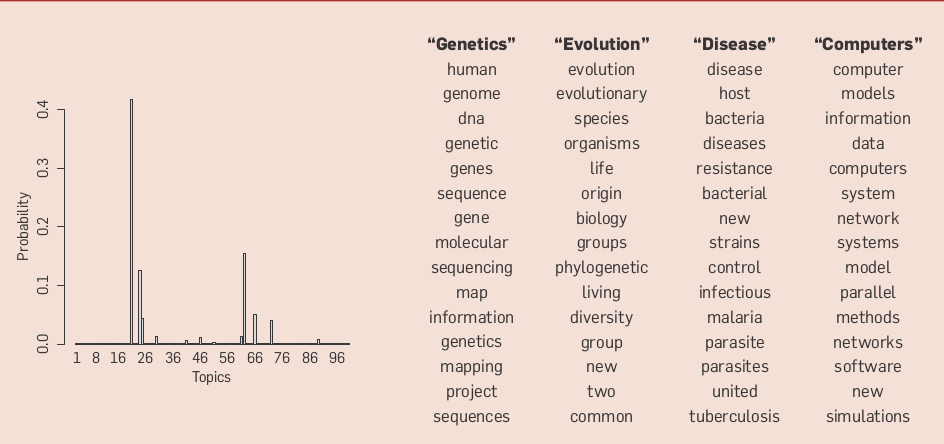
\includegraphics[scale=0.5]{infered_topics.png}
\caption{Infered topics from one article of the 17000 articles froom the journal of science.}
\label{Figure 2.2}
 \end{figure} 
\section{Graphical Model of LDA}
Figure \eqref{Figure 2.3}provides a graphical representation, showing the both the observed and latent variables involved in the generative process. The only observed part is the shaded circle $W_{d,n}$ , $\alpha$ and $\eta$ are parameters from the Diritchlet distribution.
\begin{figure}[hbtp]
\centering
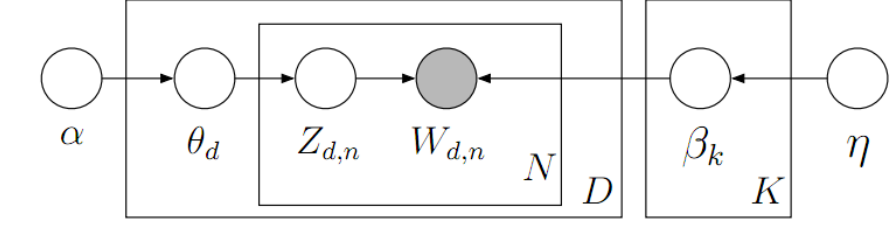
\includegraphics[scale=0.5]{Graphical.png}
\caption{Graphical representation of LDA model} \label{Figure 2.3}
\end{figure}
What the notations stands for:
\begin{itemize}
\item$D$:the number of documents
\item$N$: number of words in each document
\item$K$: number of topics
\item$\theta_d$: the topic proportion for each document $d$.
\item $Z_{d,n}$: is the topic assignment for word $n$ in document $d$.
\item $W_{d,n}$: is the observed worn $n$ in document $d$,
\item $\beta_K$:topics
\end{itemize}
From \eqref{Figure 2.3} the joint  distribution or the total probability of both latent and observed variables is given by:
\begin{align}
P(\beta,\theta,Z,W, \alpha, \beta )=\prod_{k=1}^{K}P(\beta_i)\prod_{d=1}^{D}P(\theta_d)
\prod_{n=1}^{N}P(Z_{d,n}|\theta_d)P(W_{d,n}|\beta_k,Z_{d,n})
\end{align}
\section{Diritchlet Distribution}
It is from the exponential family of continuous multivariate probability with the parameter $\alpha$ of positive real. It is denoted by $D(\alpha)$
Let $S=[S_1,S_2,...,S_d] $ as probability mass function, implies $S_i\leqslant 0$ for $i=0,1,2,,...,d$ and $\sum _{i=1}^{d}S_i$. Also suppose $\alpha=[\alpha_1,\alpha_2,...,\alpha_d]$ with $\alpha_i>0$ for each $i$, and let $\alpha_0=\sum _{i=1}^{d}\alpha_i$. Then $S$ is said to have a Dirithchlet distribution
with parameter $\alpha$, which is denoted by $S \backsim $Dir($\alpha$), if it has $f(s,\alpha)=0$, if$s$ is not a pmf and if $s$ is a pmf then,
\begin{align}
f(s,\alpha)=\frac{\Gamma(\alpha_0)}{\prod_{i=1}^{d}\Gamma(\alpha_i)}\prod_{i=1}^{d}s^{\alpha_i -1}
\end{align}
where $\Gamma()$ is the Gamma distribution.
\section{Advantages of LDA} 
LDA can be used as a module in other complex models to achieve undertake complicated tasks.
The LDA model is used in other applications, not only in text.In recent work we have used pairs of LDA modules to
model relationships between images and their corresponding descriptive captions (Blei and Jordan,2002). But also include problems involving collections of data, including data from domains such as collaborative filtering,
content-based image retrieval and bioinformatics.
\section{Disadvantages of LDA}
The bag of words assumption (the order words in a document does not matter) of LDA makes it unrealistic, however it is reasonable if only our task is to uncover the course thematic structure of the texts (Blei,2012).
\section{Extentions of LDA}
Wallach (2006) developed a model that does not ignore the assumption that the order of words does not matter (bag of words). His work uses the combination of the n gram statistic and latent topic variable by extension of the uni-gram topic model to include properties of a hierarchical Dirichlet language model.
Griffiths et al(2005) combined the idea of syntactic and semantics to produce a generative model. This model  is capable of simultaneously finding syntactic classes and semantic topics despite having no knowledge of syntax or semantics beyond statistical dependency
%Text text text text text text text text text text text text text text
%text text text text text text text text text text text text text text.
%
%When you get stuck, don't panic. 
%The world is unlikely to end just now. 
%Remember you can consult your supervisor, tutor, and Blaise at agreed times. 
%
%\begin{thm}[Jeff's Washing Theorem]
%\label{thm:jwt}
%If an item of clothing is too big, then washing it makes it bigger;
%but if it is too small, washing it makes it smaller.
%\end{thm}
%\begin{proof}
%Stated without proof. But a proof would look like this. 
%\end{proof}
%
%Notice that no Lemmas are required in the proof of Theorem \ref{thm:jwt}.
